\documentclass[12pt,a4paper]{article}

\usepackage[T1]{fontenc}
\usepackage[utf8]{inputenc}

\usepackage[english]{babel}
\usepackage{csquotes}

\usepackage[authordate-trad,backend=biber]{biblatex-chicago}
\usepackage{amsmath}
\usepackage{circuitikz}
\usepackage{mathtools}
\usepackage{todonotes}
\addbibresource{jabref.bib}

%opening
\title{By how far have recent churn-reduction techniques improved quality of experience in peer-to-peer video streaming environments?}
\author{Martin Symons}

\begin{document}

\maketitle

\begin{abstract}
abstract !!! 
\end{abstract}

\section{Introduction} \label{introduction}
Within the past ten years, video streaming traffic across the internet has exploded. Traditional client-server architectures places a large load on the small portion of nodes controlled by the streaming host, and lead to dramatic infrastructure costs. To combat this, peer-to-peer systems have been proposed that spread usage across the network's collective resources. Starting with Coolstreaming in 2004, these networks became defacto for IPTV streaming, especially pirated streams. With their utility proven, research accelerated, in pace and complexity. Industry, however, did not pick up. Since the shutdown of New Coolstreaming and PPLive in the late 2000's, these newer solutions have seen little real-world usage.

As such, the actual impact of current research on network performance is vague. Still, research since has suggested that churn has a substantial and exponential impact on client quality-of-service (QoS) beyond that which was considered in these original models. This paper investigates several marked improvements over the best-documented benchmark architecture, New Coolstreaming, with particular focus on methods to reduce churn throughout the network. wordsw words words and a list of what we discuss

\section{Literature Review}  \label{litreview}
\subsection{Peer-to-Peer Streaming Fundamentals} \label{litreview:fundamentals}
Video streaming introduces a large number of real-time requirements not seen in traditional P2P systems. File-sharing is the most popular kind of P2P network, maintaining a x\% share of internet traffic \todo{cite}. In such a network, QoS is measured mostly against upload speed, and by extension bandwidth utilization. Any intermediate action from loading a file's hash to completion is irrelevant.

playoutdeadlines startupdelay end-to-enddelay

explain the structure of our lit review - heustics first then discussing the building blocks [defined in this section] then actual implementations we will be using

\subsection{Performance Heuristics and Churn} \label{litreview:heuristics}
explaining the heuristics we use to measure how well the above requirements, and then why churn feeds into them all

\subsection{Overlay Structure} \label{litreview:structure}
Streaming systems can be mostly split into two categories, tree-based and mesh-based. Early P2P streaming networks were designed with the expectation of a rise in IP multicast uptake amongst peers. this sucks but this source \cite{Ghoshal2007} has more chunkyspread also contains citations for this

Following this, designers moved to building tree overlays across the traditional networking stack. Tree overlays are structured, with each node forwarding the complete data stream to a number of children originating from a single server at the top of all nodes. \cite{Goh2013} finds through comparative simulations that playback delay in a tree structure is up to 114\% lower than in a mesh, observing similar improvement in frame-loss ratio. We doubt the validity of these results, however - the paper proposes playback delays much shorter than the RTT of even a single hop in trees of up to 1000 nodes. Still, it is generally understood that tree overlays perform better in delay statistics that than their mesh counterparts, as the tree quickly widens as its height increases. \todo{cite} This comes at the expense of enormous susceptibility to peer churn, since a departing peer temporarily detaches all child nodes from the tree until the overlay recovers (\cite{Ghoshal2007}). The uplink bandwidth at each node in a tree also acts as a bottleneck for all children. If any one node cannot transfer the full description as necessary for playout between its children, no alternative source is available for retrieval, and QoS will suffer throughout the remaining tree (\cite{Magharei2007}).

Multi-tree networks have been proposed to mitigate this effect. Video is split into multiple substreams, each transmitted into an independently managed tree. A peer can join as many trees as necessary to meet playout demand, limited only by its download bandwidth. Since a downstream node retrieves the complete encoding from multiple parents, a single failing node no longer has catastrophic impact on its children. If a layered encoding method is chosen, playout may not even buffer, only degrade in quality. Analysis at the time suggested these topologies traded reliability and churn resistance for a more complex design and intensive media decoding requirements (\cite{Ghoshal2007}). The former is not a concern for a production network; the latter has since been resolved by the proliferation of advanced hardware video decoding chips and the integration of layered encoding in \textit{de facto} codecs like H.264. We would now consider that a multi-tree overlay represents a guaranteed improvement over single-tree.

Still, mesh networks have become the norm in recent developments. Mesh networks form a randomly connected unstructured overlay of parent-child relationships. Each node holds multiple parents and multiple children. This resembles a multi-tree; however, nodes can now freely move anywhere in the swarm, using any other node as a source for blocks, without regard for the wider network structure. Churn recovery is thus bolstered even further, and nodes can easily move away from any detected bottleneck on a given substream (\cite{Magharei2006}). Simulation results in \cite{Magharei2007} suggest bandwidth utilization in mesh networks is universally superior to a tree approach, remaining beyond 90\% in all experiments, whilst tree approaches are less efficient and more sensitive to improperly tuned parameters. This leads to at least one additional quality level being received at each node even under ideal tuning. Utilization is also shown to trough significantly under churn in a tree, whilst remaining high in a mesh. We consider these results more reliable than those presented earlier in support of tree networks - Magharei is a respected opinion in overlay construction, being cited within a number of influential papers, and has provided unbiased insight into the field's nuances across their whole portfolio.

In our paper, we only consider mesh networks due to their well-supported performance under a variety of conditions, and their resistance to churn proving relevant to our priorities. That said, hybrid networks combining tree, multi-tree and mesh networks at once have been proposed. A sweeping analysis of these toplogies proves unhelpful due to the wide range of approaches seen in the field. As such, we discuss only the performance of relevant hybrids on a per-network basis later in section \ref{litreview:monoliths}.

\subsection{Peer Selection Strategies} \label{litreview:selection}
Peer selection strategies can be split into three types: random, QoS-aware and locality-aware (\cite{Kim2018}). Random selection methods are highly resilient to churn and provide inherent load balancing \todo{we should replace this source with something About random} (\cite{Wang2013}). This may be true, other issues arise. Popular 2010's network \textit{PPLive} was noted to suffer very high startup delay. This delay was caused by a failure to quickly accrue quality nodes - the first random batch usually contained nodes with insufficient bandwidth or whom cannot be reached due to network constraints. After 150 seconds, nodes only connected to four parents \cite{Hei2008}. PPLive's popularity proves that this approach can be sufficient, but alternatives should be considered.

QoS-aware methods prioritize nodes by some network heuristic before supplying for connection. OCals tests RTT both during construction and during scheduling by proxy through TCP-Friendly Rate Control (\cite{Floyd2000}), passing equal candidates for which the new node can provide good QoS as for those providing good QoS to the node. Compared to established random selection strategy SCAMP, startup delay remains approximately constant whilst average throughput increases 103\% in a 1000 node network. Gossiped heuristics can also provide system benefit. Nodes under Chameleon (\cite{Nguyen2010}) are bootstrapped with random nodes by SCAMP; the overlay then moves nodes matching a heuristic against the requested \textit{quality level} closer together. Senders within these nodes are then selected based on matching upload/download bandwidth and lowest available layer count. This strategy massively improves playout rate at scale \todo{is this the right term?} whilst boosting quality satisfaction up to 24.7\% in smaller networks, when compared to a simpler bandwidth-based mechanism FABALAM (\cite{Liu2004}).

Locality-aware methods are the black sheep of this herd, primarily aiding underlay efficiency instead of overlay performance. They reduce end-to-end delays to a minimal, though lack the churn-resilience and throughput utilization better provided by QoS or even random approaches (\cite{Zhao2012}). Fluid representations of the selection strategy categories proved that locality-aware methods can push better performance in networks with universally high RTT (\cite{CoutodaSilva2011}), though this is a rarity in today's highly capable networks. \cite{Magharei2014} proposes OLIVE, explicitly aiming to reduce demand on the underlying routing hardware and support the best-effort internet. Though this is a valiant effort, compromises to playout quality for the sake of such optimizations are
unlikely to see uptake until a minimum QoS barrier is crossed.

Improvements originating in selection strategy choice can be amplified by exercising the strategy as wherever possible across the network. \cite{Budhkar2017} proposes three unique sorting algorithms across the network. At entry, the origin node prioritizes peers with high upload bandwidth and a full buffer. Entering nodes filter this list further by their locally perceived upload, propagation delay, lag and buffer before initiating connections. Throughout a node's lifetime, a final strategy compares all ancestors to slowly drive performance as playout continues. This thorough application of principles reduces startup delay by 10\% in all cases, and playback delay and recovery time by up to 20\% under churn. This may incur additional performance costs local to each node - however, modern hardware should be capable of these calculations without meaningful strain.

\subsection{Chunk Schedulers} \label{litreview:schedulers}
Chunk schedulers under mesh topologies are generally split into pull, push and hybrid-push-pull approaches, depending on which node takes responsibility of chunk selection. Whilst most aspects of P2P live streaming have been thoroughly surveyed, insights into the ideal scheduler approach appear limited to suppositions made in the proposal of new overlays, and a complete survey remains an open research question.

Pull schemes run the scheduler on the child node to request blocks from its parents, updated from time to time with the status of their buffer maps. The process of neighbor selection, buffer map reception, chunk selection, request and finally delivery adds up under this approach, resulting in high end-to-end delay (\cite{Hei2008a}); therefore, whilst most early overlays incorporate this basic idea, they are rarely proposed for low-latency real-time use (\cite{Zhang2007}). Under mathematical modelling, it is proven that pull schemes provide near-optimal playout probability as long as a node is allowed to push at least three blocks per timestep (\cite{Zhang2014}). Duplication is not an issue, as nodes control exactly when and how each block is received (\cite{LoCigno2008}). Generally speaking, pull schemes are considered "good enough" - even when effort is spent to determine the ideal scheme, \cite{Liang2009} finds through real-world internet experiments that the chunk scheduler only becomes relevant when both the streaming rate approaches maximum throughput for a network and minimal end-to-end delay is desired. This opinion is expressed in part by Liu, an essential figure in the field \todo{find the dissertation we need to talk about this?}

Regardless, push schemes have seen some uptake. Under this arrangement, the scheduler is run on the parent node to automatically push received blocks to its children, who attach or leave the parent at will based on their own heuristics. The children, however, have no say in the blocks that they receive. Parents must run an algorithm to determine which block should be pushed to which peer, for which many solutions have been proposed - \cite{Massoulie2007} finds through fluid modelling that the \textit{most deprived peer, random useful chunk} algorithm provides ideal throughput, whilst \cite{Sanghavi2006} theoretically proves the optimal delay of \textit{random peer, latest blind chunk} in pursuit of a hybrid approach. \cite{Bonald2008} notes, however, that the delay performance of the former and throughput of the latter are suboptimal for use in a livestreaming environment. Through simulation and mathematical analysis, the \textit{random peer, latest useful chunk} algorithm is instead found to provide the best compromise between these factors, with new methods suggested to reduce message overhead and implementation complexity. Still, this does not appear any more optimal than the aforementioned pull schemes, whilst requiring more complex mathematical models to run.

To simplify things, hybrid-push-pull approaches allow the parent node to push received blocks as before. However, the child nodes are given autonomy to select a subset of blocks to receive, usually by splitting the video into substreams. Such an approach regards the pull mechanism primarily as a routing mechanism, reducing routing, messaging and modelling overhead, whilst maintaining the high bandwidth utilization offered by push networks (\cite{Zhang2007}). The resulting granular control is tempting for those producing monolithic, tightly-optimize overlays, as explored in \ref{litreview:monoliths}.

\subsection{Coolstreaming} \label{litreview:coolstreaming}
We now consider historic implementations of peer-to-peer streaming systems in relation to the above characteristics. An explosion in IPTV popularity in the mid-2000's lead to a great number of new networks - PPLive (\cite{PPLive}), SopCast (\cite{SopCast2019}), UUSee et al. WE ARE HERE TALK ABOUT THESE BEING CLOSEDSOURCE 

Of most relevance to our paper is DONet, commercially branded Coolstreaming (\cite{1498486}). Considered the first of its breed, Coolstreaming \cite{Xie2007} \cite{asdasd} \cite{1498486}

\subsection{Coolstreaming-Compatible Improvements} \label{litreview:specifics}
https://link.springer.com/chapter/10.1007/978-3-642-30376-0\_2
\subsection{Monolithic Single Solutions} \label{litreview:monoliths}
\section{Methodology} \label{methodology}
We aimed to pit three models against each other in various QoS tests \todo{which?} to gather specific numbers on the improvements between each. Initial tests would be run on New Coolstreaming, widely considered the last popular IPTV P2P system and a good benchmark \todo{we probably already explained this in the lit review}. We would then extend this with fitting modular improvements for further measurements. \todo{name some shit} were particular targets, because \todo{blah}. Finally, we expected to implement a monolithic model, \todo{name}, to compare the capacity of incremental improvements versus the design of a single, deeply-coupled architecture.

As a simulation environment, we chose OverSim. Its included churn mechanisms, quick-switching between simplified and realistic underlay models, and complete debugging suite eased the otherwise involved development cycle. Ejecting from OverSim to OMNET++ would also have been trivial, though was never necessary.

Statistics would be presented with the built-in OMNET++ visualization tools.

\todo{needs expansion. we could mention dates?? what do people normally put here}
\section{Implementation} \label{implementation}
We based our initial experiments on New Coolstreaming as described in \cite{Li2008}. We quickly ran into problems - whilst the paper describes the stream manager and buffer map exchange in great detail, little time is given to the membership and partnership managers. The upkeep of the \textit{mCache} with incoming peers is unspecified, as is most connection management action related to churning or failing nodes and some key equations to system function. We pushed forward and attempted to fill the blanks ourselves; the final result, whilst technically functional, invariably failed to meet playout across nodes and was in no way correspondent of New Coolstreaming's measured real-world performance.

The New Coolstreaming paper concludes its discussion on the problem modules stating \textit{"these basic modules form the base for the initial Coolstreaming system,"} and that the New Coolstreaming \textit{"has made significant changes in the design of other components."} We thus considered that these modules were holdovers from the older design, implying New Coolstreaming must be built with  DONet/Coolstreaming as groundwork. We thereby set about an implementation of this more primitive design.

The final DONet implementation completed following two weeks of work. This network was similarly not ideal, though the cause was mostly banal - New Coolstreaming strips the buffer, scheduler and related messaging completely, so we saw no need to optimize these components. More worryingly, the partnership manager collapsed quickly under even minimal churn, discussed later in . Still, this constituted enough the groundwork needed to continue.

Returning with wiser eyes, we found that our architecture did not align at all with the basic modules in New Coolstreaming. This proved troubling. As discussed later in section~\ref{problems:prodopt}, DONet has clarity problems of its own when describing parts of other systems, and we noticed that the output of these components - \textit{M}-number exchanging partners ready for video transmission - \textit{did} align with the older model. We therefore treated this as a simple faulty description, and moved on to the design of the stream manager.

The well-specified stream manager came through without a hitch, but placed new constraints on the partnership manager that our already brittle implementation could not bear. We hence designed \textit{Partnerlink}, a relationship algorithm reconciling the high-churn overlay with New Coolstreaming's low-churn subscription requirements and performance at scale. This new algorithm meshed well with the stream manager, and brought our implementation to a close.

The full development process took over a month. We were therefore not able to complete any further models or make any comparisons on QoS benefits.

\section{Results and Analysis} \label{results}
In testing, we begin with two origin nodes and join 30 client nodes over the course of 90 seconds. Nodes live on average 500 seconds before churning; we allow 300 seconds for the overlay to stabilize before a 2000 second measurement period. The 500Kbps source video is split into 10 substreams, containing blocks of one second duration. Partner and membership count \(M\) is limited to 15.

We first test our model on a simple underlay without packet dropping, bandwidth limitations or timeouts. We find that our partnership mechanism works well in this environment, averaging 14.89 partners across all nodes over the entire measurement period. No node is ever seen with below 11 partners. We also, however, find our potential partner count \(M_c\) to be the same value, as our failure mechanisms are almost never engaged in this ideal environment. We find that our model maintains a satisfactory number of parent-child relationships with an average of 9.30. Despite this, our playout is poor: \todo{there is a fucking term for this i know} only 61.58\% of blocks are received before playout time. Our efficiency is reasonable - of all received blocks, 1.92\% are duplicates and 4.645\% are outside the bounds of the receiver's buffer, almost all being too old.

We test again on a realistic underlay simulating the best-effort internet, with bandwidth limitations, packet loss and queuing. Under this environment, the partnership mechanism begins to fail: despite recording an average \(M_c\) of 12.94, our actual partner count averages 1.78. We explore this and the resultant changes made to \textit{Partnerlink} in section \ref{css:comparison}. Surprisingly, our playout performs very similarly - nodes maintain an average of 9.10 parents and a playout rate of 62.00\%. This is despite a major hit to efficiency - 6.62\% of all received blocks are now out of  bounds, and 11.9\% are now duplicates. As we believe the failure in the partnership manager activates slowly over a node's lifespan, this likely means that our partnerships are very long lived; transmitted blocks must be across relationships made before the failure. The mechanics that allow playout rate to remain so high, however, are unknown.

\section{Discussion} \label{problems}
\textit{What went wrong?} New Coolstreaming is not unique as an overlay; no features within should prove particularly challenging to implement. In this section, we explore the Coolstreaming family as a whole, and illuminate the many challenges faced in their implementation amiss in the papers themselves.

\subsection{The Coolstreaming Family Tree} \label{problems:familytree}
We have so far regarded Coolstreaming as a dyad of the mesh-pull DONet/Coolstreaming and hybrid-push-pull New Coolstreaming, proposed across two papers. The reality is not so simple. Coolstreaming is formed of two models, as described. However, they have been proposed under \textit{four} different names across \textit{four} papers:

\begin{itemize}
	\item As \textit{DONet} and \textit{Coolstreaming}, in \textit{CoolStreaming/DONet: a data-driven overlay network for peer-to-peer live media streaming} \cite{Zhang2005}
	\item As \textit{Coolstreaming}, in \textit{Coolstreaming: Design, Theory, and Practice} \cite{Xie2007}
	\item As \textit{Coolstreaming+}, in \textit{An Empirical Study of the Coolstreaming+ System} \cite{Li2007}
	\item As \textit{"the new Coolstreaming,"} in \textit{Inside the New Coolstreaming: Principles, Measurements and Performance Implications} \cite{Li2008}.
\end{itemize}

Note that the name \textit{Coolstreaming} is intended by this final paper, but \textit{The New Coolstreaming} became the colloquial model name as a result of its title. Only the first paper contains the old model we have discussed as \textit{DONet/Coolstreaming} - the others all specify \textit{New Coolstreaming}, despite the name differences.

The name \textit{Coolstreaming} legally refers both to the older \textit{DONet} model and the newer \textit{New Coolstreaming} model. The confusion that results is obvious. \cite{Kondo2014} describes the \textit{SCAMP} membership protocol, the push-pull mechanism and the bootstrap node as part of the same model, despite \textit{SCAMP} being specific to the mesh-pull \textit{DONet}. \cite{Beraldi2010} makes much the same error. \cite{Lan2011} takes \textit{DONet} as its key example of a buffer-map driven overlay, but ascribes it the synchronization method seen in \textit{New Coolstreaming}. Further examples still can be found of correct prose, but with \cite{Xie2007} being cited in \cite{Zhang2005}'s place, or vice versa.

It is interesting to note that the papers themselves appear to have issues keeping the versions straight:  \cite{Li2008} describes the stream manager and new mCache system as part of the \textit{"initial Coolstreaming system"} and replaced in \textit{"the new Coolstreaming system"}, despite all of these components being local to \textit{New Coolstreaming} only - hence our initial hesitance to visit \textit{DONet}.

This escalates considering the final three papers. \cite{Xie2007} is the canon definition of \textit{New Coolstreaming}, alongside analysis of a real-world test period to determine convergence rates, start-up delay and other overlay-specific statistics. The other papers duplicate this and add further analysis: \cite{Li2007} splits users into categories, identifying network traversal problems and their respective impact on contribution. \cite{Li2008} performs an additional simulation to identify ideal values for key system parameters.

This duplication means each paper opens with a definition of \textit{New Coolstreaming}. These are not summaries - the \textit{Coolstreaming+} specification is shortest yet still clocks in at two and a half pages. The majority of this text is word-for-word identical between papers, or at best reworded. The membership and partnership managers, though, have their specifications cut down completely, no longer parsing as a working system. For instance, connection management is resolved in \cite{Xie2007} by an off-handed mention of TCP - which includes a leaving and timeout mechanism, if specified. In the other papers, TCP is never mentioned; no other connection management is described. Mechanisms to fill the bootstrap node's \textit{mCache} alongside one key function related to playout initialization are similarly constrained to this paper, despite these papers claiming to \textit{"describe the architecture and components in the new Coolstreaming system"}.

Luckily, we appear to be the only researchers to fall into this trap. Resulting development time was certainly extended, but our criticisms of the paper and our final solution remain valid.

\subsection{What does Coolstreaming need to be?} \label{problems:what}
\todo{flow this}
The \textit{Coolstreaming} family has been replaced in production by monolithic solutions like \todo{mention wiotadiof}. \textit{Coolstreaming}'s usage now lies entirely in the research domain - used as a base for reproducible results, a testbed for new modular features or a point of comparison between larger monolithic models. In all of these cases, consistency and ease of development take priority over QoS performance.

The issues mentioned so far are a sign that \textit{Coolstreaming} was never designed for this purpose. \textit{Coolstreaming} aimed to be the leading production overlay of its time, including optimizations that were inconvenient but deemed worth the miniscule performance boost. More than this, \textit{Coolstreaming} was developed as a commercial system first and a research paper second. This may explain the missing features or heavy modifications of existing solutions - the system was still under active maintenance as the papers were written, and so work had to be quick moreso than correct.

In the next section, we introduce a new model to the \textit{Coolstreaming} family designed for research purposes, outlining our priorities and rationale in doing so.

\subsection{The Fully-Connected Network Problem} \label{problems:fcn}
Both \textit{DONet} and \textit{New Coolstreaming} make the same demands on the partnership manager: given a random partial view of the network, create and maintain at most \textit{M} connections ready for video transmission. Neither paper provides any exact information on how this should be done.

Suppose a node \textit{n} joins a network of size \textit{M + 1}. All existing nodes in the network are fully saturated with partner count \textit{M}. How can this node join the network?

\begin{figure}[!ht]
	\centering
	\resizebox{0.35\textwidth}{!}{%
		\begin{circuitikz}
			\tikzstyle{every node}=[font=\LARGE]
			\draw  (7.5,15) circle (0.75cm) node {\LARGE 4} ;
			\draw  (10,15) circle (0.75cm) node {\LARGE 4} ;
			\draw  (8.75,10) circle (0.75cm) node {\LARGE 4} ;
			\draw  (6.25,12.5) circle (0.75cm) node {\LARGE 4} ;
			\draw  (11.25,12.5) circle (0.75cm) node {\LARGE 4} ;
			\draw [short] (8.25,10.5) -- (6.75,12);
			\draw [short] (9.25,10.5) -- (10.75,12);
			\draw [short] (11,13.25) -- (10.5,14.5);
			\draw [short] (6.5,13.25) -- (7,14.5);
			\draw [short] (8.25,15) -- (9.25,15);
			\draw [short] (8.5,10.75) -- (7.75,14.25);
			\draw [short] (9,10.75) -- (9.75,14.25);
			\draw [short] (7,12.5) -- (10.5,12.5);
			\draw [short] (8,14.5) -- (10.75,13);
			\draw [short] (9.5,14.5) -- (6.75,13);
			\draw  (8.75,18.75) circle (0.75cm) node {\LARGE n} ;
			\draw [dashed] (8.5,18) -- (7.75,15.75)node[pos=0.5,fill=white]{?};
			\draw [dashed] (9,18) -- (9.75,15.75)node[pos=0.5,fill=white]{?};
			\node [font=\LARGE] at (12.5,19.25) {M = 4};
		\end{circuitikz}
	}%
	\caption{Node \textit{n} cannot easily join this fully-connected network.}
	\label{fig1}
\end{figure}

In our early \textit{DONet} implementation, we forced nodes to accept all incoming partnerships, removing an old partnership to make room. This created long chains of dropped-and-replaced partnerships before the overlay settled and worsened the impact radius of churn. The move to \textit{New Coolstreaming} came with the demand to maximize partnership lifetimes, as churn would interfere with the push mechanism and result in wasted blocks being sent to a peer, totally invalidating this approach.

Several solutions exist, though none are trivial. Our final implementation requests a node to break one partnership, placing the new partner in the middle. This has a great number of implications on the network, most notably that \textit{M} must now be divisible by 2. Since \textit{DONet} uses \textit{M = 15} as example, this cannot be the implementation as intended by the original authors.

\begin{figure}[!ht]
	\centering
	\resizebox{0.35\textwidth}{!}{%
		\begin{circuitikz}
			\tikzstyle{every node}=[font=\LARGE]
			\draw  (7.5,15) circle (0.75cm) node {\LARGE 4} ;
			\draw  (10,15) circle (0.75cm) node {\LARGE 4} ;
			\draw  (8.75,10) circle (0.75cm) node {\LARGE 4} ;
			\draw  (6.25,12.5) circle (0.75cm) node {\LARGE 4} ;
			\draw  (11.25,12.5) circle (0.75cm) node {\LARGE 4} ;
			\draw [short] (9.25,10.5) -- (10.75,12);
			\draw [short] (11,13.25) -- (10.5,14.5);
			\draw [short] (6.5,13.25) -- (7,14.5);
			\draw [short] (8.5,10.75) -- (7.75,14.25);
			\draw [short] (9,10.75) -- (9.75,14.25);
			\draw [short] (7,12.5) -- (10.5,12.5);
			\draw [short] (8,14.5) -- (10.75,13);
			\draw [short] (9.5,14.5) -- (6.75,13);
			\draw  (8.75,18.75) circle (0.75cm) node {\LARGE 4} ;
			\node [font=\LARGE] at (12.5,19.25) {M = 4};
			\draw [short] (7.5,15.75) -- (8.5,18);
			\draw [short] (10,15.75) -- (9,18);
			\draw [short] (8,18.75) .. controls (5.75,17.75) and (4.75,15.5) .. (6,13.25);
			\draw [short] (8,10) .. controls (2.75,11.5) and (2.5,17.25) .. (8,18.75);
		\end{circuitikz}
	}%
	\caption{A solved topology, as according to the pairing method.}
	\label{fig2}
\end{figure}

We can at least infer some details from \textit{DONet}. The \textit{mCache} data structure includes \textit{num\_partners} for each visible node, which is updated but never apparently used. In a healthy network, the likelihood of a node directly knowing another node with less than \textit{M} partners is low. Instead, we assume this to be part of a gossiping mechanism where a gossiped partnership request is directed towards nodes with missing partners, which would also justify the use of \textit{SCAMP} as opposed to a more standard partial view aggregator. We include a similar strategy as part of our implementation; we discuss this in detail later in section \ref{css:partnerlink:panicking}.

That said, the phrasing of the scheduled switching as established \textit{"with nodes randomly selected from [the] mCache"} implies a more direct communication. In this case, it is unknown how \textit{DONet} or \textit{New Coolstreaming} solve this problem.

\subsection{Choosing New Partners} \label{problems:newpartners}
The two inequalities measuring connection quality are also applied to any candidate partners following a detected failure. Inequality 1 limits the gap between a node's  buffers and the parent's. If we apply this to candidates after failing because of this inequality, we will filter out any nodes further ahead than our old node, slipping further back in our buffer. Assuming we never change our playout position, this new node will not be able to service our entire buffer area.

Furthermore, the nodes seen within this inequality will mostly be those similarly falling behind the swarm; that is, nodes with equally poor connections. This groups poorly performant nodes and drags them backwards across the buffers, eventually collapsing entirely. In our model we disabled inequality 1 when measuring candidates, and performance resumed - \textit{New Coolstreaming} must use some other unspecified mechanism to avoid this.

\subsection{Requesting the Block} \label{problems:requesting}
\textit{New Coolstreaming} specifies an algorithm to compare all buffer maps from a node's first partners and calculate the  to request. The method through which this is done is somewhat obscure - the subscription map only communicates on-off booleans. We assume this is achieved by manipulating the latest blocks shown to each node to suggest the node has already received up to that block, despite having just joined. This requires some careful planning to execute without triggering subscriptions from nodes but is a clever usage of the limited data structure at play.

A feature unmentioned here is the behaviour-of and restrictions-on the playout index. Neither \textit{Coolstreaming} implementation specifies a recovery mechanism - nodes are assumed to never fall completely behind the swarm. This leaves us two options - either the playout index must never buffer or pause after sync, and continue to play forward on encounter with missing blocks, or the recovery mechanism is left undefined. Given that there is a startup delay listed amongst the results, we can assume the latter. If the stream does include buffering or the node is suffering poor local performance, though, the need to recover is inevitable. There are many options for approach that impact performance, and one best solution should ideally be provided.

\subsection{Production Optimizations} \label{problems:prodopt}
\textit{DONet} defers to \textit{SCAMP} for membership connection management, \todo{we need to establish ahead of time the fanout proofs of SCAMP etc.} before overruling it on several counts. Where \textit{SCAMP} automatically adjusts membership count in sync with the size of the system, \textit{DONet} enforces a hard limit of \textit{M} nodes, usually 15. The indirection mechanism is implemented only in primitive form, with only nodes within the origin's view being available as contacts. As \textit{DONet} only uses \textit{SCAMP} to gather a random partial view, and does not use it as a means of message transmission itself, \textit{DONet} does not require \textit{SCAMP}'s full set of guarantees. Whilst we have not been able to perform experiments to prove this, we hypothesize that these restrictions therefore make no negative impact on the network, included to reduce message overhead.

Other optimizations are less successful. \textit{SCAMP} specifies a leasing system to remove dead nodes from the pool, which \textit{DONet} accepts. However, in the case that the partnership manager finds a partner that fails to send a buffer map in a given period, the partnership overrides the membership manager to remove the node from the \textit{mCache}. The partnership manager then emits a departure message on its behalf, which is gossiped \textit{"similarly to the membership message,"} i.e. once to a peer who then repeats it to every node in its \textit{mCache}. Since exactly \textit{M} departure messages are gossiped, every message would have to reach a peer knowing the failed node for a clean exit. The layers of indirections involved in membership management, however, make it unlikely for this message to reach any such peer at all.

This mechanism is applied even to departure messages sent by a leaving node itself. \textit{SCAMP} notes that each node knows the peers it is subscribed to through its \textit{InView} list - thus, the only requirement for a clean exit is to send a departure to each node it contains. The gossiped alternative makes no gain in message overhead whilst almost totally invalidating its effect on network topology.

This appears to be a malformed optimization to allow nodes to depart each other in case of failure. Even if this were successful, the already-established leasing system means any performance gain would be negligible.

Successful or not, these changes represent a problem: we fall back to some existing research solution for a problem and then brain slug \todo{is this actually a good turn of phrase} it for some slight gain, in the process tampering with that solution's proven performance. This is convenient for the original researcher, but requires careful cross-referencing of the two papers for accurate reproduction. New implementation of the model therefore becomes strenuous, and inaccuracies made much more likely.

\todo{we need to flow this}

\section{Introducing \textit{coolstreaming-spiked}} \label{css}
\textit{coolstreaming-spiked} is a new iteration of \textit{Coolstreaming} bringing the two models into synthesis. Research usage is targeted through an easier implementation, thorough central specification and compatibility with a wide range of IPTV improvements. Specifically:

\begin{itemize}
	\item The SCAMP protocol is retained for backwards compatibility with research performed on the original \textit{DONet}.
	\item The partnership connection algorithm is solved and documented as \textit{Partnerlink}, a novel approach providing realistic performance and absolutely minimal churn impact for networks of any scale.
	\item Production optimizations are stripped back to focus on a smaller scope.
	\item Other fixes, such as the disabling of inequality 1 on candidates, are implemented as standard.
\end{itemize}

We now proceed to describe the function of this model.

\subsection{Architecture} \label{css:architecture}
Our component architecture is identical to that seen in \textit{New Coolstreaming}: a membership manager provides the model with a continuous pool of random nodes. The partnership manager filters these nodes to find connections suited for video transmission, and handles the exchange of buffer maps. The stream manager creates parent-child relationships, owns the buffer and forwards blocks to peers. Each node within the architecture is provided a unique \textit{NodeID} - an IP address will suffice.

We incorporate the substream system as defined in \textit{New Coolstreaming}. The video sequence is split into blocks of equal size each assigned a timestamp sequence number. These are shared equally between \(K\)-number zero-indexed substreams, where the \textit{i}-th substream contains blocks with sequence numbers \((nK + \textit{i})\) where \(n\) is a positive integer from zero to infinity. For instance, assuming \(K = 4\), substream 2 would contain blocks with ID \(\{2, 6, 10, 14, ...\}\).

\subsection{Membership Manager} \label{css:membership}
The membership manager makes the initial contact to an origin node. We then subscribe as members to a subset of nodes using SCAMP to provide the partial view. No changes are made to SCAMP - the standard subscription, unsubscription, indirection, leasing and recovery methods all apply. There is no limit on the size of the \textit{mCache}. The partnership manager can no longer directly influence the mCache or send unsubscription messages on behalf of another node. These changes allow researchers to follow a well-specified, battle-tested paper for gossiping support without cross-referencing our own. The main output of this component is an arbitrarily sized set of random nodes across the network.

SCAMP does not describe any starting topology. A bootstrapped SCAMP network must contain at least two nodes engaged in a shared subscription.

In the case that the node ever becomes completely isolated and can no longer aggregate members, the node should recontact the origin and gossip a fresh subscription message.

\subsection{Partnership Manager and \textit{Partnerlink}} \label{css:partnerlink}
The partnership manager takes these nodes and begins to form TCP connections ready for block transmission. TCP performs the majority of connection upkeep on our behalf - if the connection ends, times out or fails, the partnership should be considered \textit{failed}. \todo{this doesn't mean anything}

The buffer map system remains as specified in \textit{New Coolstreaming}. A buffer map comprises two tuples of length \textit{K} - the first listing the highest block sequence number received in each substream, the second listing the subscription of substreams to the receiving partner. For instance, a node receiving tuples of \(\{40, 41, 42, 39\}\) and \(\{0, 0, 0, 1\}\) from a partner should infer the node to have most recently received block 39 on substream 3, and prepare a subscription for the node on that substream according to the subscription map. We also transfer the node's current \textit{panic status} and a \textit{NodeID} representing an \textit{associated peer}, discussed later in \ref{css:partnerlink:panicking} and \ref{css:stream}. A node receiving a buffer map should store these values alongside their relevant partner; the latest block should only be set if the subscription is new as of this message, as we update this value locally as part of the stream manager. If a partner does not transfer a buffer map in some specified length of time, the partner is missing and the partnership should be considered \textit{failed} - the partner connection is removed and \(M_c\) (discussed later) is reduced by 1.

\subsubsection{\textit{Partnerlink} Description} \label{css:partnerlink:description}
We now describe the \textit{Partnerlink} algorithm. We first make two constraints on the system - a maximum number of partners at each node \(M\) is introduced, where \(M\mod{2} = 0\). Our base join operation grants a node two links per request, so an even partner cap is essential. We define a starting network as two or more nodes in a valid system topology, since at least two peers are necessary to begin splitting. This basic network could be comprised of two guaranteed-trustworthy origin nodes, or built cooperatively with potentially-malicious client nodes.

\tikzset{every picture/.style={line width=0.75pt}} %set default line width to 0.75pt        

\begin{figure}[!ht]
	\centering
	\resizebox{0.25\textwidth}{!}{%
		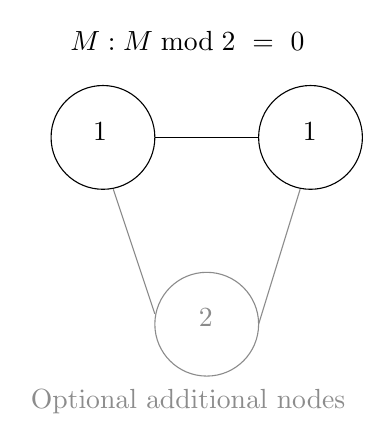
\begin{tikzpicture}[x=0.75pt,y=0.75pt,yscale=-1,xscale=1]
			%uncomment if require: \path (0,224); %set diagram left start at 0, and has height of 224
			
			%Shape: Circle [id:dp8053367545608073] 
			\draw   (360,75) .. controls (360,61.19) and (371.19,50) .. (385,50) .. controls (398.81,50) and (410,61.19) .. (410,75) .. controls (410,88.81) and (398.81,100) .. (385,100) .. controls (371.19,100) and (360,88.81) .. (360,75) -- cycle ;
			%Shape: Circle [id:dp5139832099367154] 
			\draw   (260,75) .. controls (260,61.19) and (271.19,50) .. (285,50) .. controls (298.81,50) and (310,61.19) .. (310,75) .. controls (310,88.81) and (298.81,100) .. (285,100) .. controls (271.19,100) and (260,88.81) .. (260,75) -- cycle ;
			%Straight Lines [id:da34739028917979153] 
			\draw    (310,75) -- (360,75) ;
			%Shape: Circle [id:dp7166484753359771] 
			\draw  [color={rgb, 255:red, 139; green, 139; blue, 139 }  ,draw opacity=1 ] (310,165) .. controls (310,151.19) and (321.19,140) .. (335,140) .. controls (348.81,140) and (360,151.19) .. (360,165) .. controls (360,178.81) and (348.81,190) .. (335,190) .. controls (321.19,190) and (310,178.81) .. (310,165) -- cycle ;
			%Straight Lines [id:da740820997595583] 
			\draw [color={rgb, 255:red, 139; green, 139; blue, 139 }  ,draw opacity=1 ]   (290,100) -- (310,160) ;
			%Straight Lines [id:da5098257307652958] 
			\draw [color={rgb, 255:red, 139; green, 139; blue, 139 }  ,draw opacity=1 ]   (380,100) -- (371.33,128.18) -- (360,165) ;
			
			% Text Node
			\draw (268,22.4) node [anchor=north west][inner sep=0.75pt]    {$M:M\bmod 2\ =\ 0$};
			% Text Node
			\draw (279,66.4) node [anchor=north west][inner sep=0.75pt]    {$1$};
			% Text Node
			\draw (380,66.4) node [anchor=north west][inner sep=0.75pt]    {$1$};
			% Text Node
			\draw (330,156.4) node [anchor=north west][inner sep=0.75pt]  [color={rgb, 255:red, 139; green, 139; blue, 139 }  ,opacity=1 ]  {$2$};
			% Text Node
			\draw (249,195) node [anchor=north west][inner sep=0.75pt]   [align=left] {\textcolor[rgb]{0.55,0.55,0.55}{Optional additional nodes}};
			
			
		\end{tikzpicture}
	}%
	\caption{The base topology from which \textit{Partnerlink} must operate.}
	\label{fig3}
\end{figure}

Each node tracks an additional set of variables. We maintain a set of \textit{locks} against \textit{NodeID}s for which operations are still in progress, to protect the system when a node receives several requests regarding the same node. We also maintain an \textit{anticipated} partner count \(M_c\), tracking what our partner count will become if all ongoing operations resolve successfully. Making decisions against this value rather than our actual partner count ensures we do not accidentally request partners above our hard limit \(M\).

\textit{Partnerlink} operations can be split into three categories:
\begin{itemize}
	\item \textbf{Initiation}, allowing a healthy node to create new connections with known nodes.
	\item \textbf{Management}, allowing the overlay to adapt after a failed partnership.
	\item \textbf{Panic}, allowing an unhealthy node to recover back to \(M\) connections.
\end{itemize}
We now discuss the systems and messages in place to allow for these operations.

\subsubsection{\textit{Partnerlink} Initiation} \label{css:partnerlink:initiation}
A node \(n\) entering the network for the first time awaits the first \textit{SCAMP Inview} message to initialize the \textit{Partnerlink} manager. A list of up to \(M / 2\) candidate partners is requested from the contained node, retrieved at random from its \textit{mCache}. This is necessary as the local node's \textit{mCache} needs time to fill with peers; relying on it for first partners comes with substantial startup delay.
Upon reception at node \textit{n}, these nodes are all locked and sent a \textit{Split} message. This performs the split operation discussed prior, attempting to place the node in-between an existing partnership. The node also sets \(M_c\) to \(M_r * 2\), where \(M_r\) is the number of nodes received from the initial exchange. A node \(a\) receiving a \textit{Split} message checks that no partnership nor lock is held against \(n\) - if not, the node forwards a \textit{TrySplit} message to a random unlocked partner \(b\), holding locks against it and \(n\). Node \(b\) performs the same checks, additionally requiring that \(a\) is not locked. If the checks pass, it returns a \textit{TrySplitSuccess} message, breaks the connection with its old partner and initiates with the new node. Node \(a\) receiving a \textit{TrySplitSuccess} breaks the connection similarly and unlocks the two nodes, after which the exchange is complete. Upon connection, node \(n\) removes its lock on node \(a\). The newly joined node has now gained two links, breaking only one in the process. If all \textit{Split} messages respond successfully, the node will have created exactly \(M\) partnerships.

If node \(b\) fails its checks, it responds a \textit{TrySplitFailure}. If node \(a\) receives a \textit{TrySplitFailure}, fails its own checks or does not know another unlocked partner, a \textit{SplitFailure} is forwarded back to the new node \(n\) which reduces \(M_c\) by 2 and unlocks the contacted node. This causes the node to immediately begin panicking.

\subsubsection{\textit{Partnerlink} Panicking} \label{css:partnerlink:panicking}
If a node does not satisfy \(M_c = M\), it is described as \textit{panicking}. A node checks its panic state after each update to \(M_c\). We begin to look for alternative ways to create new links in the system.

If \(M_c = M - 1\), we cannot fill our empty partners by splitting, as we would breach our limit. We instead gossip a 
\textit{Panic} message containing our \textit{NodeID} to a random partner. This message is directed across the network towards panicking nodes with priority, as determined from their buffer maps. Otherwise, the message is directed towards any node that is not the original panicking node or the last hop. Otherwise, the message is directed anywhere, or else dropped. If a panicking node receives a \textit{Panic} message, it initiates a connection with the contained node and increases its \(M_c\) by 1. The original node receiving this connection does the same, unless it has since stopped panicking, in which case it rejects the connection.

This joins two panicking nodes together directly and grants one new link each. This is mostly effective in very small networks, where nodes impacted by an improper exit are very few hops together. As networks grow and stabilize, the hops between panicking nodes will increase, worsening delay before node recovery. Note that locks do not influence the transmission of this message, as its result on a partner does not influence a node's local link count.

If \(M_c = M - 2\), we fall back to the splitting method. We gossip a \textit{PanicSplit} message containing our \textit{NodeID} to a random partner. This message contains a field \textit{LastHopOpinion}, initialized to \textit{CANT\_HELP}. The same direction mechanism is applied, although with priority now given to non-panicking nodes and a ban on gossiping to locked partners. If a node receives a \textit{PanicSplit} with \textit{LastHopOpinion CANT\_HELP}, the node performs similar checks as in a regular \textit{Split} - that we are not already partnered with nor hold any locks against the contained node. If the checks pass, the message is gossiped to a random unlocked partner with a \textit{LastHopOpinion} \textit{CAN\_HELP}, and the contained node and random partner are locked; else, it is marked \textit{CANT\_HELP}.

If a node receives a \textit{PanicSplit} with \textit{LastHopOpinion CAN\_HELP}, we perform the same checks with an additional check that we do not hold a lock against the last hop node. If these checks fail, we throw a \textit{PanicSplitFailed} back to the last hop, who unlocks the contained node and partner. We then recurse and treat the message as if \textit{LastHopOpinion} had been \textit{CANT\_HELP}. If these checks pass, we proceed as if from a successful \textit{TrySplit} - a \textit{PanicSplitSuccess} is gossiped back to the last hop, our partnership with it is closed and a new connection is initiated with the contained node. The node receiving the \textit{PanicSplitSuccess} message switches connections similarly. The panicking node receiving the connections increases \(M_c\) by 1 each, unless it has since stopped panicking, in which case it rejects the connection.

This finds two relatively stable nodes within the network and places the panicking node between them. This is mostly effective in large networks, where the gossiped message will quickly find its way to nodes with no knowledge of the sender. In networks with node count \(Nc \leq M + 1\), this message will never resolve. The resolution rate quickly improves from there.

If \(0 < M_c \leq M - 3\), we gossip both of the above messages at once.

If \(M_c = 0\), we should assume major disturbance amongst our membership peers. The standard SCAMP leave procedure should be followed to cleanly disconnect from the membership network in the membership manager, before recontacting the origin to gather a fresh partial view and begin new partnerships from scratch.

Each of the above messages contains a time-to-live which is checked at each receiving node. If this timeout expires, the message is dropped. It is the responsibility of each panicking node to resend messages after they time out.

These messages are gossiped to partners, though they could instead be gossiped to members. We suspect that gossiping to partners will bias recipients towards those with a larger number of partnerships (i.e. those with more stable connections) allowing for more effective recovery, whereas the \textit{mCache} may contain a greater concentration of already-poor connections. We cannot provide any proof of this theory, however - this would prove a fruitful future research question.

\subsubsection{\textit{Partnerlink} Leaving} \label{css:partnerlink:leaving}
To avoid unneeded panics when disconnecting a node, it is intuitive to pair nodes back together, undoing the splitting we performed to enter. If we perform this via messaging, however, failing nodes will still panic all of their nodes, adding \(M\) panicking nodes to the network - a substantial overlay breakdown. Instead, we continually inform nodes of their \textit{associated peer} when exchanging buffer maps. A clean leave then commands nodes to switch connections to the node they have already been informed of, and nodes detecting timeouts or a failing node can switch automatically without external assistance. This mechanism allows for overlay repair without any gossiped messages in most cases.

Nodes should be associated deterministically - that is, for as long as a node holds the same partners, the associated peer for each partner should not change. Given a set of partners \{A, B, C, ...\}, the associated peer for A is B, and for B is A. If there is an odd number of partners, the final peer is associated with an exceptional \textit{NodeID} to be caught later. Peers receiving a buffer map should store the new associated peer corresponding to this partnership, replacing any prior peer. If the partnership fails or times out, the node should first attempt to connect to their associated peer. If this connection fails, or the node was associated with the exceptional \textit{NodeID}, the node should reduce \(M_c\) by 1, entering a panic state.

A leaving node should send a \textit{Leave} message to each of its peers before ending the connection. Each receiving node should then immediately attempt the above procedure regardless of the state of the partnership.

\subsubsection{\textit{Partnerlink} Switching} \label{css:partnerlink:switching}
\textit{coolstreaming-spiked} is designed for compatibility with both \textit{DONet} and \textit{New Coolstreaming} research models. To provide this support, we retain the switching system unique to \textit{DONet}. At a set interval, each node should perform a standard \textit{Switch} procedure on a random node in its \textit{mCache}, without changing \(M_c\). Two randomly-chosen associated partners should be locked. If both new links are successful, these two partners should be sent \textit{Leave} messages, so that they reconnect to each other; else, the procedure is abandoned and the two partners are unlocked.

\subsubsection{\textit{Partnerlink} Rationale} \label{css:partnerlink:rationale}
The \textit{Split} and \textit{Panic} messages are near-identical to those hypothesized to act within the \textit{DONet} model. Switching could also not be achieved without some similar mechanism. These are essential items  for the minimum output required of the partner component. The \textit{SplitPanic} system primarily acts as a caution against early failure when connecting to initial candidate partners. One downside of the \textit{Split} model is the chance of collisions - there is some chance that two candidates contact the same node to perform two splits. Network conditions may also lead to a node being impossible to contact. In either case, it is not unreasonable to expect a large number of contacted nodes to be unreachable, resulting in a starting \(M_c\) far below \(M\), which would take a long time to recover with the vanilla \textit{Panic} strategy. Whilst performance is not a priority for this model, there is still a minimum bar beyond which research analysis would become clouded by its limitations; starting delay is one such case.

The new \textit{associated peers} model is ultimately easier to implement than the \textit{de facto} leave method associated with a splitting approach. Nodes would have to associate peers and forward them to nodes regardless, with the addition of some special case for nodes leaving without notification. The model also grants extra opportunities for filtering \todo{however we phrase this is determined by our lit review}. Thus, we consider this approach an improvement over the immediately obvious solution.

Whilst the switching mechanism does provide compatibility, its impact on the model is limited compared to the more integral role the \textit{mCache} takes in replacing partners in \textit{DONet}. Research surrounding peer selection algorithms will therefore appear less impactful under \textit{coolstreaming-spiked} - a more in-depth port may also include the algorithm as part of the \textit{associated peer} system to accentuate the impact it makes.

\subsection{Stream Manager} \label{css:stream}
The stream manager is responsible for converting partnerships to parent-child subscriptions, pushing data around as necessary, as well as the dissemination of buffer maps.

Each node regularly emits a buffer map to every partner. The syntax of these maps has already been discussed - however, an exception on valid syntax is made for when the node has just entered the network. Once buffer maps have been received from some defined minimum percentage of partners, the node must calculate an ideal starting index based on the known set of latest received blocks. Designating \(H_{{S_i},A}\) as the latest block received block for substream \(S_i\) at node \(A\), the starting index at substream \(i\) is calculated as \[I_{S_i} = \max\{H_{{S_i},q} : q \in partners\} - T_p\] where \(T_p\) is a constant to be introduced later. The ideal placement of the starting playout index is specific to the playout strategy and is an open research question. We expect that buffering systems should place playout at \(\min\{I_{S_i}\}\) and begin playout once a minimum buffer percentage has been filled. Non-buffering approaches are more complicated - playout should be placed such this buffer percentage will have been filled by the time playout reaches \(\min\{I_{S_i}\}\). The ideal calculation for this remains an open research question and will likely require additional information to be gossiped between nodes.

When pushing buffer maps to partners when it has not yet received blocks in a given substream \textit{i}, a new node should fill its latest block with some exceptional value, either a manually-filtered \textit{null} or a very large negative number to ensure the node is never selected, unless the node intends to make its first subscription on \textit{i} to that partner. In this case, the latest block on this substream should be listed as \(I_{S_i} - K\) to ensure the partner's stream manager begins transmission from the relevant point.

When a node \(n\) subscribes to a substream through their buffer map, the partnership manager reads and stores the node's latest received block \(R_n\). The manager attends to each subscribing partner with a round-robin strategy. At each step, if the node's buffers contains block with sequence number \(R_n + K\), the manager pushes this block to node \(n\) and updates \(R_n\) accordingly, moving on to the next node. The stream manager should aim to fully saturate a node's outgoing bandwidth - as soon as one block finishes transmission, the next should begin. The stream manager will continue to push all blocks in the substream until the partnership or subscription ends; a parent node will not drop a child under any other circumstance.

For monitoring the service of substream \(j\) to child node \(A\) by parent \(p\), two inequalities are defined

\begin{flalign}
\max\{|H_{{S_i},A} - H_{{S_j},p}| : i \leq K\} < T_s \\
\max\{|H_{{S_i},q}| : q \in partners\} - H_{{S_j},p} < T_p
\end{flalign}

Inequality (1) caps the distance between the most up-to-date child substream and the target parent substream. If this inequality does not hold, the parent has blocks we are interested in that we are not receiving, implying issues with the link. Inequality (2) caps the distance between the target parent substream and the most up-to-date substream we know across all partners. If this inequality does not hold, the parent is lagging behind the wider swarm, implying connection issues further upstream. At each buffer map and block reception, these inequalities are measured against each substream parent - if either fail, the parent is reselected. The replacement parent is selected randomly from all other partners meeting inequality (2) for the target substream - if no partner meets the inequality, the reselection is cancelled. If any reselection occurs, a new buffer map is immediately sent to the affected parents. A cooldown timer \(T_i\) is set on a per-substream basis to prevent repeated reselection and stabilize the overlay topology. Substreams with active cooldowns will not be checked.

The failure state for the stream manager depends on playout strategy. If buffering is incorporated, the node may fall behind the blocks available in the wider swarm. If playout does not halt, we may still find ourselves in a situation where all partners provide unsatisfactory connections. A number of heuristics could detect either case; a threshold over the filled percentage of the buffer is one simple example. Whatever the method, the stream manager should assume a widespread failure amongst its underlying partners, and initiate the same recovery mechanism as defined in the partnership manager.

\subsection{Comparison of \textit{coolstreaming-spiked} to our implementation} \label{css:comparison}
Our implementation discussed prior is \textit{not} an implementation of \textit{coolstreaming-spiked}, though they are basically similar. The key differences are

\begin{itemize}
	\item Our implementation retains the \textit{DONet} version of \textit{SCAMP}, with all its oddities. We do not anticipate this aspect of the system to have any impact on performance, and the component outputs are the same.
	\item Our implementation does not include any locking mechanism - instead, more advanced link counting is used to resolve overlapping message streams without hiding nodes from overlay adjustment. The interactions that arise are nearly impossible to reason and are very likely the reason for the desyncing \(M_c\) and partner counts we note in our results. The locking mechanism is proposed due to our experiences with this other approach. This will have an impact on results, though almost certainly a positive one.
	\item Our implementation does not make any use of TCP connections, instead relying on UDP either directly or through \textit{OverSim}'s RPC support. This is related both to the cut-down paper we worked from and that TCP support in \textit{OverSim} is a somewhat hidden feature. This negatively impacts our results, as TCP networking is essential in the design of \textit{Coolstreaming}.
	\item Our implementation initiates playout similarly to a buffering playout strategy, syncing to the starting block index and waiting for a threshold percentage of the buffer to be filled to play. No other buffering is performed during playout. This strange hybrid approach, whilst not invalid, is unlikely to be seen in a real research model and would ideally instead align with one or the other.
\end{itemize}

The changes we have made to \textit{coolstreaming-spiked} since our implementation aim to resolve the poor performance seen in our results. Whilst the final performance figures are unverified, we believe this to be a good future vein of research.

\section{Conclusion} \label{conclusion}
holy fuck. this sucks

\printbibliography
\end{document}
